\section{Blockschema}

\paragraph{Syftet med blockschema}
Blockschema är ett systematisk sätt att rita reglerade system på.

\paragraph{Hur funkar det?}
Betrakta blocket i figur \ref{fig:basic_block}.

\begin{figure}[!ht]
	\centering
	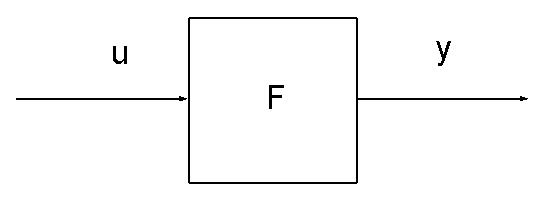
\includegraphics[width = 0.5\textwidth]{./Images/basic_block.eps}
	\caption{Illustration av ett enkelt block i ett blockschema.}
	\label{fig:basic_block}
\end{figure}

Med denna figuren menar vi exakt att $Y(s) = F(s)U(s)$.